% Options for packages loaded elsewhere
\PassOptionsToPackage{unicode}{hyperref}
\PassOptionsToPackage{hyphens}{url}
%
\documentclass[
]{book}
\usepackage{amsmath,amssymb}
\usepackage{iftex}
\ifPDFTeX
  \usepackage[T1]{fontenc}
  \usepackage[utf8]{inputenc}
  \usepackage{textcomp} % provide euro and other symbols
\else % if luatex or xetex
  \usepackage{unicode-math} % this also loads fontspec
  \defaultfontfeatures{Scale=MatchLowercase}
  \defaultfontfeatures[\rmfamily]{Ligatures=TeX,Scale=1}
\fi
\usepackage{lmodern}
\ifPDFTeX\else
  % xetex/luatex font selection
\fi
% Use upquote if available, for straight quotes in verbatim environments
\IfFileExists{upquote.sty}{\usepackage{upquote}}{}
\IfFileExists{microtype.sty}{% use microtype if available
  \usepackage[]{microtype}
  \UseMicrotypeSet[protrusion]{basicmath} % disable protrusion for tt fonts
}{}
\makeatletter
\@ifundefined{KOMAClassName}{% if non-KOMA class
  \IfFileExists{parskip.sty}{%
    \usepackage{parskip}
  }{% else
    \setlength{\parindent}{0pt}
    \setlength{\parskip}{6pt plus 2pt minus 1pt}}
}{% if KOMA class
  \KOMAoptions{parskip=half}}
\makeatother
\usepackage{xcolor}
\usepackage{color}
\usepackage{fancyvrb}
\newcommand{\VerbBar}{|}
\newcommand{\VERB}{\Verb[commandchars=\\\{\}]}
\DefineVerbatimEnvironment{Highlighting}{Verbatim}{commandchars=\\\{\}}
% Add ',fontsize=\small' for more characters per line
\usepackage{framed}
\definecolor{shadecolor}{RGB}{248,248,248}
\newenvironment{Shaded}{\begin{snugshade}}{\end{snugshade}}
\newcommand{\AlertTok}[1]{\textcolor[rgb]{0.94,0.16,0.16}{#1}}
\newcommand{\AnnotationTok}[1]{\textcolor[rgb]{0.56,0.35,0.01}{\textbf{\textit{#1}}}}
\newcommand{\AttributeTok}[1]{\textcolor[rgb]{0.13,0.29,0.53}{#1}}
\newcommand{\BaseNTok}[1]{\textcolor[rgb]{0.00,0.00,0.81}{#1}}
\newcommand{\BuiltInTok}[1]{#1}
\newcommand{\CharTok}[1]{\textcolor[rgb]{0.31,0.60,0.02}{#1}}
\newcommand{\CommentTok}[1]{\textcolor[rgb]{0.56,0.35,0.01}{\textit{#1}}}
\newcommand{\CommentVarTok}[1]{\textcolor[rgb]{0.56,0.35,0.01}{\textbf{\textit{#1}}}}
\newcommand{\ConstantTok}[1]{\textcolor[rgb]{0.56,0.35,0.01}{#1}}
\newcommand{\ControlFlowTok}[1]{\textcolor[rgb]{0.13,0.29,0.53}{\textbf{#1}}}
\newcommand{\DataTypeTok}[1]{\textcolor[rgb]{0.13,0.29,0.53}{#1}}
\newcommand{\DecValTok}[1]{\textcolor[rgb]{0.00,0.00,0.81}{#1}}
\newcommand{\DocumentationTok}[1]{\textcolor[rgb]{0.56,0.35,0.01}{\textbf{\textit{#1}}}}
\newcommand{\ErrorTok}[1]{\textcolor[rgb]{0.64,0.00,0.00}{\textbf{#1}}}
\newcommand{\ExtensionTok}[1]{#1}
\newcommand{\FloatTok}[1]{\textcolor[rgb]{0.00,0.00,0.81}{#1}}
\newcommand{\FunctionTok}[1]{\textcolor[rgb]{0.13,0.29,0.53}{\textbf{#1}}}
\newcommand{\ImportTok}[1]{#1}
\newcommand{\InformationTok}[1]{\textcolor[rgb]{0.56,0.35,0.01}{\textbf{\textit{#1}}}}
\newcommand{\KeywordTok}[1]{\textcolor[rgb]{0.13,0.29,0.53}{\textbf{#1}}}
\newcommand{\NormalTok}[1]{#1}
\newcommand{\OperatorTok}[1]{\textcolor[rgb]{0.81,0.36,0.00}{\textbf{#1}}}
\newcommand{\OtherTok}[1]{\textcolor[rgb]{0.56,0.35,0.01}{#1}}
\newcommand{\PreprocessorTok}[1]{\textcolor[rgb]{0.56,0.35,0.01}{\textit{#1}}}
\newcommand{\RegionMarkerTok}[1]{#1}
\newcommand{\SpecialCharTok}[1]{\textcolor[rgb]{0.81,0.36,0.00}{\textbf{#1}}}
\newcommand{\SpecialStringTok}[1]{\textcolor[rgb]{0.31,0.60,0.02}{#1}}
\newcommand{\StringTok}[1]{\textcolor[rgb]{0.31,0.60,0.02}{#1}}
\newcommand{\VariableTok}[1]{\textcolor[rgb]{0.00,0.00,0.00}{#1}}
\newcommand{\VerbatimStringTok}[1]{\textcolor[rgb]{0.31,0.60,0.02}{#1}}
\newcommand{\WarningTok}[1]{\textcolor[rgb]{0.56,0.35,0.01}{\textbf{\textit{#1}}}}
\usepackage{longtable,booktabs,array}
\usepackage{calc} % for calculating minipage widths
% Correct order of tables after \paragraph or \subparagraph
\usepackage{etoolbox}
\makeatletter
\patchcmd\longtable{\par}{\if@noskipsec\mbox{}\fi\par}{}{}
\makeatother
% Allow footnotes in longtable head/foot
\IfFileExists{footnotehyper.sty}{\usepackage{footnotehyper}}{\usepackage{footnote}}
\makesavenoteenv{longtable}
\usepackage{graphicx}
\makeatletter
\newsavebox\pandoc@box
\newcommand*\pandocbounded[1]{% scales image to fit in text height/width
  \sbox\pandoc@box{#1}%
  \Gscale@div\@tempa{\textheight}{\dimexpr\ht\pandoc@box+\dp\pandoc@box\relax}%
  \Gscale@div\@tempb{\linewidth}{\wd\pandoc@box}%
  \ifdim\@tempb\p@<\@tempa\p@\let\@tempa\@tempb\fi% select the smaller of both
  \ifdim\@tempa\p@<\p@\scalebox{\@tempa}{\usebox\pandoc@box}%
  \else\usebox{\pandoc@box}%
  \fi%
}
% Set default figure placement to htbp
\def\fps@figure{htbp}
\makeatother
\setlength{\emergencystretch}{3em} % prevent overfull lines
\providecommand{\tightlist}{%
  \setlength{\itemsep}{0pt}\setlength{\parskip}{0pt}}
\setcounter{secnumdepth}{5}
\usepackage{booktabs}
\usepackage[]{natbib}
\bibliographystyle{plainnat}
\usepackage{bookmark}
\IfFileExists{xurl.sty}{\usepackage{xurl}}{} % add URL line breaks if available
\urlstyle{same}
\hypersetup{
  pdftitle={Advanced Research Writing in Statistics and Data Science},
  pdfauthor={Kun Chen},
  hidelinks,
  pdfcreator={LaTeX via pandoc}}

\title{Advanced Research Writing in Statistics and Data Science}
\author{Kun Chen}
\date{2025-08-21}

\usepackage{amsthm}
\newtheorem{theorem}{Theorem}[chapter]
\newtheorem{lemma}{Lemma}[chapter]
\newtheorem{corollary}{Corollary}[chapter]
\newtheorem{proposition}{Proposition}[chapter]
\newtheorem{conjecture}{Conjecture}[chapter]
\theoremstyle{definition}
\newtheorem{definition}{Definition}[chapter]
\theoremstyle{definition}
\newtheorem{example}{Example}[chapter]
\theoremstyle{definition}
\newtheorem{exercise}{Exercise}[chapter]
\theoremstyle{definition}
\newtheorem{hypothesis}{Hypothesis}[chapter]
\theoremstyle{remark}
\newtheorem*{remark}{Remark}
\newtheorem*{solution}{Solution}
\begin{document}
\maketitle

{
\setcounter{tocdepth}{1}
\tableofcontents
}
\chapter*{Preface}\label{preface}
\addcontentsline{toc}{chapter}{Preface}

This book aims to train students in statistics and data science on academic
writing with professional tools such as LaTeX, BibTeX, R, and Git.

This book is currently under-development, and it is meant to be
an extended version of the book ``Statistical Writing'' \url{https://github.com/statds/stat-writing} written by Dr.~Elizabeth Schifano and Dr.~Jun Yan.

The notes are prepared with the \textbf{bookdown} R package \citep{xie2016bookdown},
which can be installed from CRAN or Github:

\begin{Shaded}
\begin{Highlighting}[]
\FunctionTok{install.packages}\NormalTok{(}\StringTok{"bookdown"}\NormalTok{)}
\CommentTok{\# or the development version}
\CommentTok{\# devtools::install\_github("rstudio/bookdown")}
\end{Highlighting}
\end{Shaded}

Remember each Rmd file contains one and only one chapter, and a chapter is
defined by the first-level heading \texttt{\#}.

To compile this example to PDF, you need XeLaTeX. You are recommended to install
TinyTeX (which includes XeLaTeX): \url{https://yihui.name/tinytex/}.

\chapter{Introduction}\label{intro}

What does a statistical or data science paper look like? As with all scientific papers, it should have some commonly expected structures: title, abstract, keywords, introduction, methods, results, discussion, acknowledgements, references, appendix, and supplement. Due to the specificity of the statistical discipline, machine learning practices, and application domains, however, research papers can look very different from one another.

\begin{center}\rule{0.5\linewidth}{0.5pt}\end{center}

\section{Types of Statistical Papers}\label{types-of-statistical-papers}

\subsection{Theory papers}\label{theory-papers}

A \textbf{theory paper} in statistics and probability is closest in form to a mathematical paper. It typically includes the statement of the problem, formulation of assumptions, and the presentation of theorems, lemmas, and proofs. The purpose is often to establish fundamental properties of certain statistical or probabilistic tools/approaches, including but well beyond consistency, efficiency, optimality, convergence, asymptotic distributions, and non-asymptotic error bounds.

While theory papers may not always feature data, simulations, or applications, they form the \textbf{mathematical and probabilistic foundation} upon which methodology and applied work are built.

Most of the articles in journals such as \emph{Annals of Statistics}, \emph{Annals of Probability}, \emph{Bernoulli}, \emph{Probability Theory and Related Fields}, among others, are considered as theory papers. In other words, these journals should be the primary outlets for a theory paper.

Examples include \citet{Foygel2021}.

\subsection{Method papers}\label{method-papers}

A \textbf{method paper} focuses on proposing a novel methodological contribution that can be applied to a general class of real-world problems. A commonly seen structure is:

\begin{itemize}
\tightlist
\item
  Introduction\\
\item
  Methods (e.g., estimation, hypothesis tests, diagnostic procedures)\\
\item
  Theoretical properties\\
\item
  Simulation studies\\
\item
  Applications/illustrations\\
\item
  Discussion/Conclusions
\end{itemize}

Such papers often include a blend of theory (e.g., asymptotic guarantees) and empirical validation. See, for example, \citet{li2023regularized}; \citet{lau2022bias}.

\subsection{Applied papers}\label{applied-papers}

An \textbf{applied paper} focuses on addressing a concrete scientific question in a particular domain using statistical or data science methods. Its structure often includes:

\begin{itemize}
\tightlist
\item
  Introduction\\
\item
  Data description\\
\item
  Methods (applied or adapted)\\
\item
  Results\\
\item
  Discussion
\end{itemize}

Sometimes simulation studies are added to assess sensitivity. Applied papers may involve applying existing methods or developing new ones motivated by the application. Examples include \citet{price2022effects}; \citet{caplan2019dental}; \citet{jiao2022cyberattack}.

\begin{center}\rule{0.5\linewidth}{0.5pt}\end{center}

\section{Data Science and Machine Learning Papers}\label{data-science-and-machine-learning-papers}

Beyond traditional statistics journals, researchers often publish in \textbf{data science and machine learning outlets} such as \emph{NeurIPS}, \emph{ICML}, \emph{KDD}, and \emph{AAAI}. These papers emphasize:

\begin{itemize}
\tightlist
\item
  Conciseness (strict page limits)\\
\item
  Algorithmic novelty\\
\item
  Benchmark comparisons on standard datasets\\
\item
  Open-source reproducibility\\
\item
  Clarity for an interdisciplinary readership
\end{itemize}

Compared to \emph{JASA} or \emph{Annals of Statistics}, these outlets prioritize \textbf{empirical performance and novelty} over lengthy theoretical development, though many still include core mathematical analysis.

\begin{center}\rule{0.5\linewidth}{0.5pt}\end{center}

\section{Audience and Purpose}\label{audience-and-purpose}

An author should always keep the \textbf{target audience} in mind. Statistical journals span a wide spectrum from applied to theoretical. Machine learning venues differ again in expectations. Even technical reports, white papers, or grant proposals have unique readerships. Regardless of outlet, any scientific writing should be convincing and concise. Authors must show that their work is important, valid, and useful --- and avoid wasting the reader's time.

\begin{center}\rule{0.5\linewidth}{0.5pt}\end{center}

\section{Scientific Writing Resources}\label{scientific-writing-resources}

Many resources on scientific writing are available. For example, \citet{gopen1990science} was selected by its publisher, \emph{American Scientist}, as one of its 36 ``Classic Articles'' from the first 100 years of publishing history. Popular books are \citet{oshima2000writing}, \citet{gopen2004expectations}, \citet{hairston2003successful}, and \citet{lebrun2021scientific}.

\begin{center}\rule{0.5\linewidth}{0.5pt}\end{center}

\section{About This Book}\label{about-this-book}

This book, \emph{Advanced Research Writing in Statistics and Data Science}, extends earlier efforts such as \href{https://statds.github.io/stat-writing/}{\emph{stat-writing}} by broadening the scope to include not only statistical research writing but also writing for \textbf{data science and machine learning communities}.

The book emphasizes three guiding principles:

\begin{enumerate}
\def\labelenumi{\arabic{enumi}.}
\tightlist
\item
  \textbf{Clarity and Persuasion} -- communicating complex technical ideas to both expert and interdisciplinary audiences.\\
\item
  \textbf{Genre Awareness} -- tailoring style and structure to journals, conferences, and other outlets.\\
\item
  \textbf{Learning by Doing} -- the book includes examples, annotated excerpts, and practical exercises.
\end{enumerate}

\begin{center}\rule{0.5\linewidth}{0.5pt}\end{center}

\section{Outline of the Book}\label{outline-of-the-book}

The planned content includes:

\begin{itemize}
\tightlist
\item
  \textbf{Introduction} (this chapter): Types of research papers and outlets.\\
\item
  \textbf{Clarity and Conciseness}: Avoiding jargon, redundancy, and ambiguity.\\
\item
  \textbf{Titles, Abstracts, and Introductions}: Crafting compelling entry points.\\
\item
  \textbf{Methods and Results}: Presenting technical material effectively.\\
\item
  \textbf{Figures, Tables, and Captions}: Communicating visually.\\
\item
  \textbf{Discussion and Conclusions}: Framing contributions and limitations.\\
\item
  \textbf{Peer Review and Revision}: Writing reviews, responding to reviewers, revising.\\
\item
  \textbf{Grant Proposals and Research Statements}: Writing beyond papers.\\
\item
  \textbf{Ethics and Integrity}: Authorship, plagiarism, and responsible use of AI.\\
\item
  \textbf{Exercises and Practice}: Rewriting, reviewing, and polishing tasks.
\end{itemize}

Each chapter will include \textbf{examples drawn from real papers across statistics, biostatistics, and machine learning} and will feature \textbf{exercises} that mimic the real writing and review process.

\chapter{Introduction}\label{introduction}

What does a statistical paper look like? As with all scientific papers, it
should have some commonly expected structures which include components such as
title, abstract, keywords, introduction, methods, results, discussion,
acknowledgements, references, appendix, and supplement. Due to the
specificity of the statistical discipline and application areas, however,
statistical papers could look quite different one from another.

There are different types of statistical papers. A theory paper would look
similar to a paper in mathematics, with statement of the problem, presentation
of some theorems, and technical proofs. Such papers are not covered here. We
focus on two types of statistical papers: application papers and method papers.
Application papers focus on a specific application problem in a certain domain
where the research discoveries depend on applications of existing or novel
statistical methods. Method papers, on the other hand, aim to provide a general
methodological solution to a class of applied problems. Often, methods
paper have a theoretical component, for example, the establishment of the
asymptotic properties of a new estimator. An applied paper in statistics could
be a method paper in the domain of the problem it solves.

An author should always keep the target audience in mind when writing. There are
many statistical journals on the wide spectrum from applied to theoretical
papers. Each one has its own aims and scope, with different target
readerships. Writings such as customary statistical reports that are not
intended for journal publications also have target readerships. Regardless of
the audience, any scientific paper should be convincing and concise. You need to
show the readers that your work is important, valid, and useful. You don't want
to waste the time of any readers.

\section{Applied papers}\label{applied-papers-1}

An applied paper has a widely accepted structure:

\begin{itemize}
\tightlist
\item
  Introduction
\item
  Data description
\item
  Methods
\item
  Results
\item
  Discussion
\end{itemize}

An applied paper can be applying existing statistical methods to solve an
applied problem. See, for example, \citet{price2022effects}; \citet{caplan2019dental}.

When sensitivity analysis is desired for the applications, one can have a
section on simulation studies. See, for example, \citet{jiao2022cyberattack};
\citet{li2021uncertainty}.

Some applied papers can involve novel methodology development that is motivated
by an applied problem. In such cases, simulation studies become necessary, where
you validate your methods with simulated data so you can check your estimator
with the truth. Such check is not feasible when analyzing real data.
See, for example, \citet{jiao2021bayesian}; \citet{hu2021moving}.

\section{Methods papers}\label{methods-papers}

A methods paper focuses on a novel method that is applicable to a general class
of problems arising in different domains. A commonly seen structure is:

\begin{itemize}
\tightlist
\item
  Introduction
\item
  Methods (e.g., estimation, hypothesis tests, diagnosis)
\item
  Properties
\item
  Simulations
\item
  Illustrations (with real applications)
\item
  Discussion/Conclusions.
\end{itemize}

The simulations section is often needed for methods papers. Any method has
assumptions. Any reasonably good method should work as expected when the
assumptions hold. It would be even better if it remains working when some of the
assumptions are violated. Simulation studies can be designed to check whether
the proposed estimators are unbiased and more efficient than competing
estimators; whether the proposed tests retains their sizes and are more powerful
than competing tests.

Here are some examples: \citet{li2023regularized}; \citet{lau2022bias}.

\section{Scientific Writing}\label{scientific-writing}

Many resources on scientific writing are available. For example,
\citet{gopen1990science} was selected by its publisher, \emph{American Scientist},
as one of its 36 ``Classic Articles'' from the first 100 years of its
publishing history. Popular books are
\citet{oshima2000writing}, \citet{gopen2004expectations}, \citet{hairston2003successful},
and \citet{lebrun2021scientific}.

\chapter{Cross-references}\label{cross}

Cross-references make it easier for your readers to find and link to elements in your book.

\section{Chapters and sub-chapters}\label{chapters-and-sub-chapters}

There are two steps to cross-reference any heading:

\begin{enumerate}
\def\labelenumi{\arabic{enumi}.}
\tightlist
\item
  Label the heading: \texttt{\#\ Hello\ world\ \{\#nice-label\}}.

  \begin{itemize}
  \tightlist
  \item
    Leave the label off if you like the automated heading generated based on your heading title: for example, \texttt{\#\ Hello\ world} = \texttt{\#\ Hello\ world\ \{\#hello-world\}}.
  \item
    To label an un-numbered heading, use: \texttt{\#\ Hello\ world\ \{-\#nice-label\}} or \texttt{\{\#\ Hello\ world\ .unnumbered\}}.
  \end{itemize}
\item
  Next, reference the labeled heading anywhere in the text using \texttt{\textbackslash{}@ref(nice-label)}; for example, please see Chapter \ref{cross}.

  \begin{itemize}
  \tightlist
  \item
    If you prefer text as the link instead of a numbered reference use: \hyperref[cross]{any text you want can go here}.
  \end{itemize}
\end{enumerate}

\section{Captioned figures and tables}\label{captioned-figures-and-tables}

Figures and tables \emph{with captions} can also be cross-referenced from elsewhere in your book using \texttt{\textbackslash{}@ref(fig:chunk-label)} and \texttt{\textbackslash{}@ref(tab:chunk-label)}, respectively.

See Figure \ref{fig:nice-fig}.

\begin{Shaded}
\begin{Highlighting}[]
\FunctionTok{par}\NormalTok{(}\AttributeTok{mar =} \FunctionTok{c}\NormalTok{(}\DecValTok{4}\NormalTok{, }\DecValTok{4}\NormalTok{, .}\DecValTok{1}\NormalTok{, .}\DecValTok{1}\NormalTok{))}
\FunctionTok{plot}\NormalTok{(pressure, }\AttributeTok{type =} \StringTok{\textquotesingle{}b\textquotesingle{}}\NormalTok{, }\AttributeTok{pch =} \DecValTok{19}\NormalTok{)}
\end{Highlighting}
\end{Shaded}

\begin{figure}

{\centering 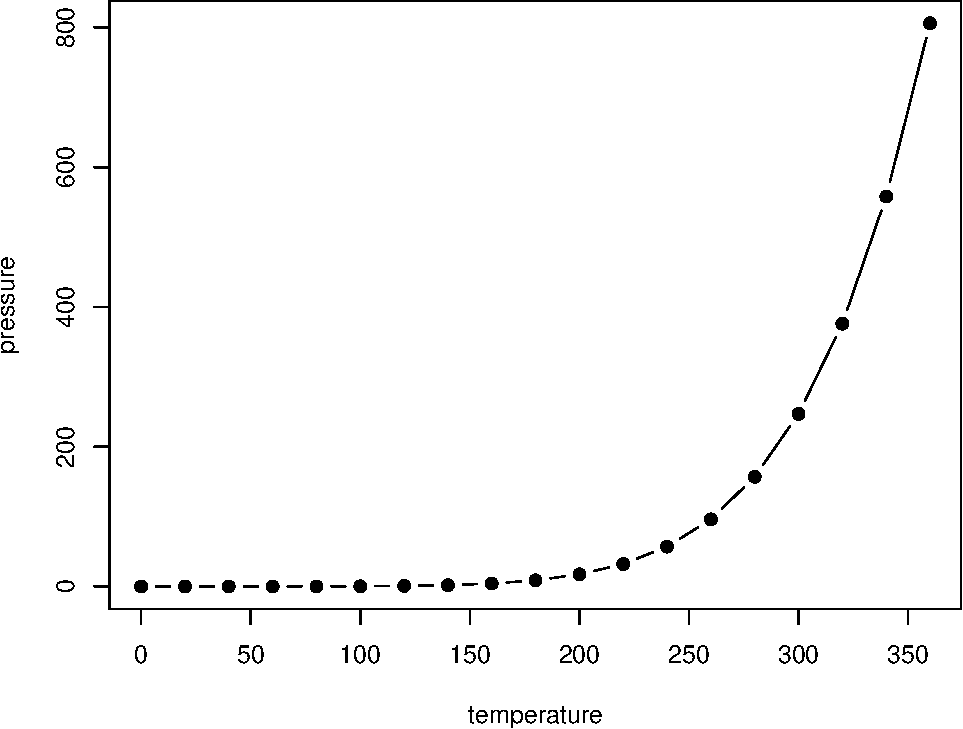
\includegraphics[width=0.8\linewidth,alt={Plot with connected points showing that vapor pressure of mercury increases exponentially as temperature increases.}]{_main_files/figure-latex/nice-fig-1} 

}

\caption{Here is a nice figure!}\label{fig:nice-fig}
\end{figure}

Don't miss Table \ref{tab:nice-tab}.

\begin{Shaded}
\begin{Highlighting}[]
\NormalTok{knitr}\SpecialCharTok{::}\FunctionTok{kable}\NormalTok{(}
  \FunctionTok{head}\NormalTok{(pressure, }\DecValTok{10}\NormalTok{), }\AttributeTok{caption =} \StringTok{\textquotesingle{}Here is a nice table!\textquotesingle{}}\NormalTok{,}
  \AttributeTok{booktabs =} \ConstantTok{TRUE}
\NormalTok{)}
\end{Highlighting}
\end{Shaded}

\begin{table}

\caption{\label{tab:nice-tab}Here is a nice table!}
\centering
\begin{tabular}[t]{rr}
\toprule
temperature & pressure\\
\midrule
0 & 0.0002\\
20 & 0.0012\\
40 & 0.0060\\
60 & 0.0300\\
80 & 0.0900\\
\addlinespace
100 & 0.2700\\
120 & 0.7500\\
140 & 1.8500\\
160 & 4.2000\\
180 & 8.8000\\
\bottomrule
\end{tabular}
\end{table}

\chapter{Parts}\label{parts}

You can add parts to organize one or more book chapters together. Parts can be inserted at the top of an .Rmd file, before the first-level chapter heading in that same file.

Add a numbered part: \texttt{\#\ (PART)\ Act\ one\ \{-\}} (followed by \texttt{\#\ A\ chapter})

Add an unnumbered part: \texttt{\#\ (PART\textbackslash{}*)\ Act\ one\ \{-\}} (followed by \texttt{\#\ A\ chapter})

Add an appendix as a special kind of un-numbered part: \texttt{\#\ (APPENDIX)\ Other\ stuff\ \{-\}} (followed by \texttt{\#\ A\ chapter}). Chapters in an appendix are prepended with letters instead of numbers.

\chapter{Footnotes and citations}\label{footnotes-and-citations}

\section{Footnotes}\label{footnotes}

Footnotes are put inside the square brackets after a caret \texttt{\^{}{[}{]}}. Like this one \footnote{This is a footnote.}.

\section{Citations}\label{citations}

Reference items in your bibliography file(s) using \texttt{@key}.

For example, we are using the \textbf{bookdown} package \citep{R-bookdown} (check out the last code chunk in index.Rmd to see how this citation key was added) in this sample book, which was built on top of R Markdown and \textbf{knitr} \citep{xie2015} (this citation was added manually in an external file book.bib).
Note that the \texttt{.bib} files need to be listed in the index.Rmd with the YAML \texttt{bibliography} key.

The RStudio Visual Markdown Editor can also make it easier to insert citations: \url{https://rstudio.github.io/visual-markdown-editing/\#/citations}

\chapter{Blocks}\label{blocks}

\section{Equations}\label{equations}

Here is an equation.

\begin{equation} 
  f\left(k\right) = \binom{n}{k} p^k\left(1-p\right)^{n-k}
  \label{eq:binom}
\end{equation}

You may refer to using \texttt{\textbackslash{}@ref(eq:binom)}, like see Equation \eqref{eq:binom}.

\section{Theorems and proofs}\label{theorems-and-proofs}

Labeled theorems can be referenced in text using \texttt{\textbackslash{}@ref(thm:tri)}, for example, check out this smart theorem \ref{thm:tri}.

\begin{theorem}
\protect\hypertarget{thm:tri}{}\label{thm:tri}For a right triangle, if \(c\) denotes the \emph{length} of the hypotenuse
and \(a\) and \(b\) denote the lengths of the \textbf{other} two sides, we have
\[a^2 + b^2 = c^2\]
\end{theorem}

Read more here \url{https://bookdown.org/yihui/bookdown/markdown-extensions-by-bookdown.html}.

\section{Callout blocks}\label{callout-blocks}

The R Markdown Cookbook provides more help on how to use custom blocks to design your own callouts: \url{https://bookdown.org/yihui/rmarkdown-cookbook/custom-blocks.html}

\chapter{Sharing your book}\label{sharing-your-book}

\section{Publishing}\label{publishing}

HTML books can be published online, see: \url{https://bookdown.org/yihui/bookdown/publishing.html}

\section{404 pages}\label{pages}

By default, users will be directed to a 404 page if they try to access a webpage that cannot be found. If you'd like to customize your 404 page instead of using the default, you may add either a \texttt{\_404.Rmd} or \texttt{\_404.md} file to your project root and use code and/or Markdown syntax.

\section{Metadata for sharing}\label{metadata-for-sharing}

Bookdown HTML books will provide HTML metadata for social sharing on platforms like Twitter, Facebook, and LinkedIn, using information you provide in the \texttt{index.Rmd} YAML. To setup, set the \texttt{url} for your book and the path to your \texttt{cover-image} file. Your book's \texttt{title} and \texttt{description} are also used.

This \texttt{gitbook} uses the same social sharing data across all chapters in your book- all links shared will look the same.

Specify your book's source repository on GitHub using the \texttt{edit} key under the configuration options in the \texttt{\_output.yml} file, which allows users to suggest an edit by linking to a chapter's source file.

Read more about the features of this output format here:

\url{https://pkgs.rstudio.com/bookdown/reference/gitbook.html}

Or use:

\begin{Shaded}
\begin{Highlighting}[]
\NormalTok{?bookdown}\SpecialCharTok{::}\NormalTok{gitbook}
\end{Highlighting}
\end{Shaded}


  \bibliography{book.bib,packages.bib,6694.bib}

\end{document}
